\documentclass[a4paper, 10pt]{report}
\usepackage[italian]{babel}
\usepackage[T1]{fontenc}
\usepackage[utf8]{inputenc}
\usepackage{charter}
\usepackage{amsmath}
\usepackage{amsthm}
\usepackage{amsfonts}
\usepackage{graphicx}
\usepackage{wrapfig}
\usepackage{tcolorbox}
\usepackage{fancyhdr}
\usepackage{listings}
\usepackage{longtable}

\usepackage{geometry}
\geometry{a4paper, left=2cm,right=2cm,top=2cm,bottom=2cm}

\pagestyle{fancy}
\lhead{}
\chead{}
\rhead{\bfseries 07 - 13 novembre 2019 }
\lhead{\bfseries Segnali e immagini}

\begin{document}
\subsection*{Trasformata di Fourier}
\paragraph*{Trasformata} Sia $f(t)$ un segnale continuo su $f: R \rightarrow R$, anche non periodico. Si chiama trasformata di Fourier $\mathfrak{F}(f(t)) = F(\mu)$ il segnale $\mathfrak{F} : R \rightarrow C$:
\begin{align*}
\mathfrak{F}(f(t)) = F(\mu) = \int_{-\infty}^{+\infty} f(t)e^{-j2\pi \mu t} \, dt
\end{align*}
\noindent dove $\mu$ rappresenta l'angolo $\frac{n}{T}$ della serie di Fourier. La trasformata esiste se il segnale $f(t)$ è di energia (se il segnale è di energia può comunque avere trasformata).

\noindent In pratica, la trasformata restituisce un coefficiente di presenza $F(\mu)$ per la frequenza $\mu$. Se $f(t)$ è reale, la sua trasformata è generalmente complessa, dove:
\begin{itemize}
\item[-] Se $t$ rappresenta il tempo, $\mu$ rappresenta gli Hertz (cicli/secondi);
\item[-] Se $t$ rappresenta lo spazio, $\mu$ rappresenta la frequenza spaziale (cicli/metri).
\end{itemize}
\noindent Gli spettri di fase e ampiezza qui diventano continui o continui a tratti.

\begin{center}
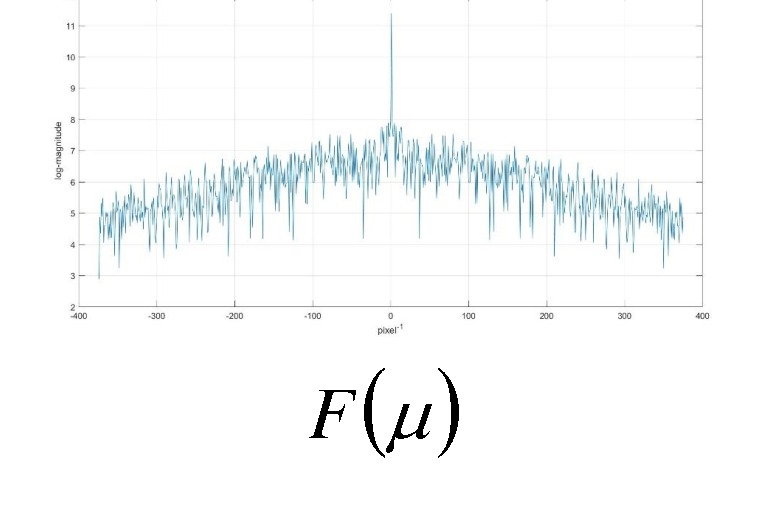
\includegraphics[scale=0.4]{2.pdf}
\end{center}

\paragraph*{Antitrasformata} Sia $F(\mu)$ la trasformata di Fourier di un segnale $f: R \rightarrow R$. Si dice trasformata inversa di Fourier il segnale 
\begin{align*}
\mathfrak{F}^{-1}(F(\mu)) = f(t) = \int_{-\infty}^{+\infty} F(\mu)e^{j2\pi \mu t} \, d\mu
\end{align*}
\noindent L'antitrasformata permette di ricostruire $f$ a partire da $F$.

\begin{center}
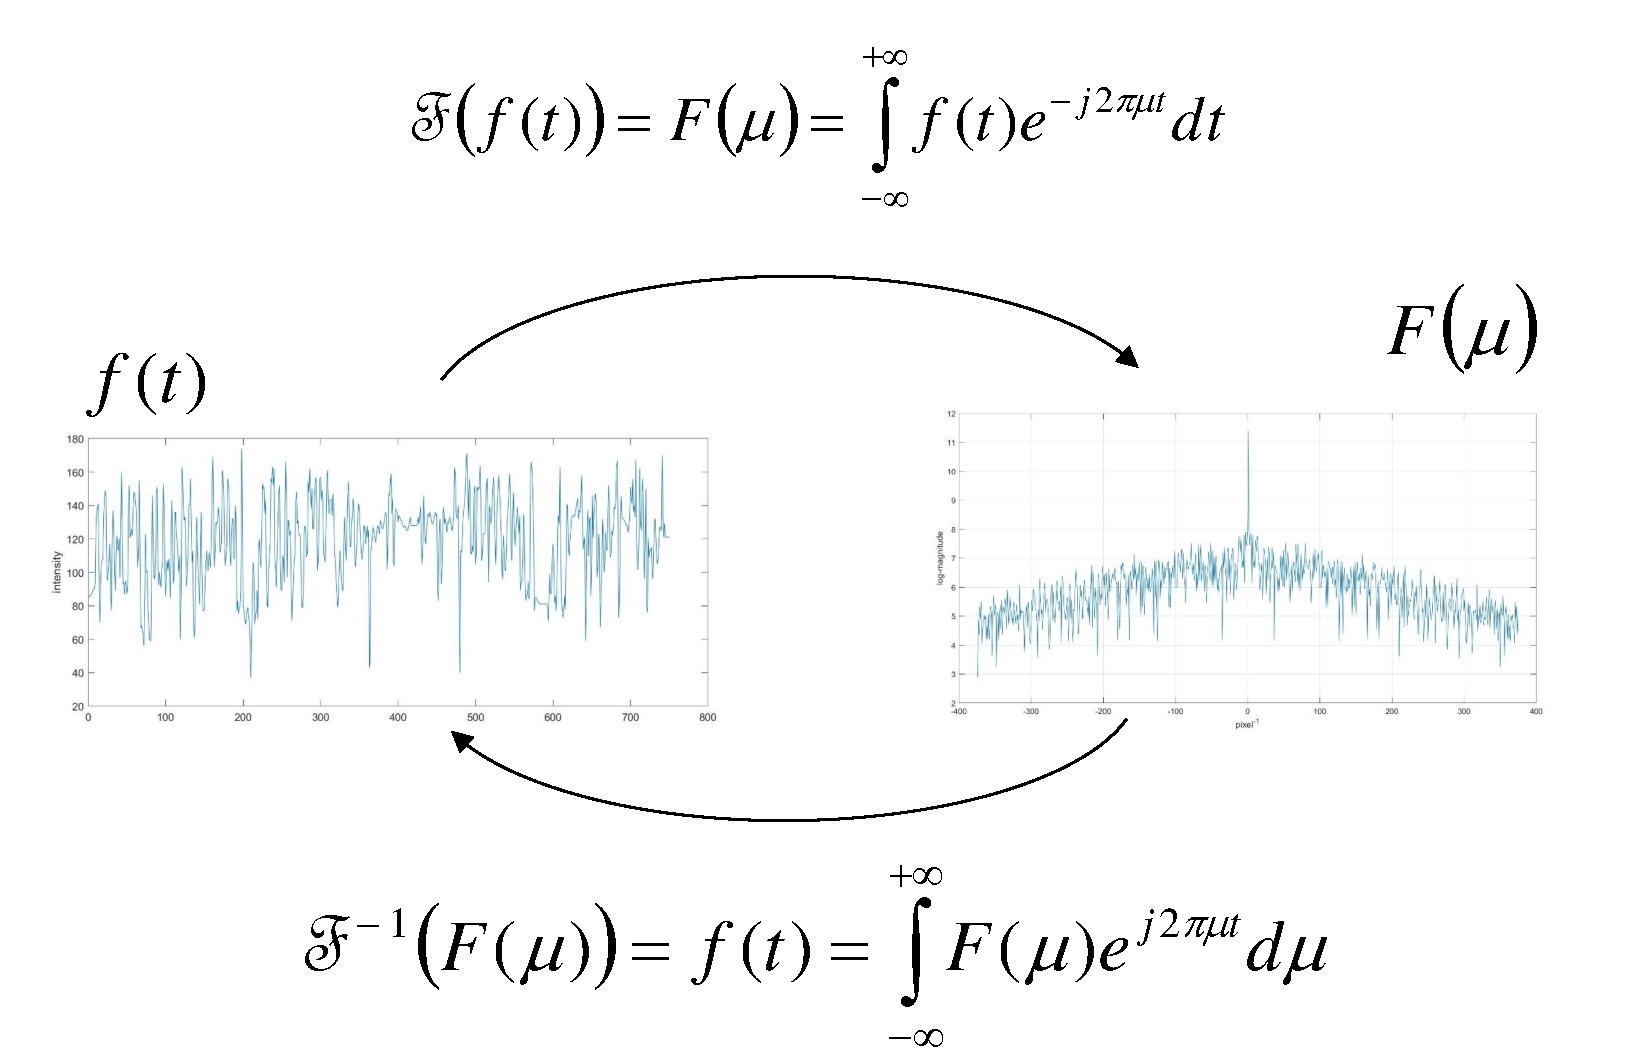
\includegraphics[scale=0.4]{1.pdf}
\end{center}

\paragraph*{Proprietà della trasformata} Le proprietà della trasformata di Fourier sono:
\begin{longtable}{ p{.30\textwidth}  p{.60\textwidth} }
\textbf{Linearità} & $a_1f_1(t) + a_2f_2(t) -> a_1F_1(\mu) + a_2F_2(\mu)$ 
\\\\
\textbf{Scalatura temporale} & $z(t) = f(at) -> Z(\mu) = \frac{1}{a}F(\frac{\mu}{a})$
\\\\
\textbf{dualità} & $f(t) -> F(\mu)$
\\
 & $F(t) -> f(-\mu)$
\end{longtable}

\paragraph*{Funzione sinc}
La trasformata di Fourier della box generica è:\\
\begin{align*}
\mathfrak{F}\left(f(t)\right) = F(\mu) &= \int^{+\infty}_{-\infty}A\Pi \left(\frac{t}{w}e^{-j 2 \pi \mu t}\right) \, dt \\
&= \int^{+\frac{w}{2}}_{-\frac{w}{2}} A e^{-j 2 \pi \mu t} \, dt \\
& = ... \\
&= \frac{A}{\pi \mu} sin(\pi \mu w) \\
&= Aw \frac{sin(\pi \mu w)}{\pi \mu w} \hspace{0.5cm}\text{FUNZIONE SINC}
\end{align*}

\noindent In generale, la funzione sinc è definita come segue:
\begin{align*}
sinc(m) = \frac{sin(\pi m)}{\pi m} \hspace{1cm}\text{dove}\hspace{1cm} sinc(0) = 1, sinc(m) = 0
\end{align*}

\paragraph*{Trasformata di un Impulso} La trasformata di Fourier di un generico impulso è la seguente:

\begin{align*}
\mathfrak{F}(f(t)) = F(\mu) &= \int^{+\infty}_{-\infty} \delta(t) e^{-j2 \pi \mu t} \, dt\\
&= \int^{+\infty}_{-\infty} \delta(0) e^{-j2 \pi \mu 0} \, dt\\
&= 1
\end{align*}

\noindent La trasformata genera quindi una costante. Nel caso l'impulso sia centrato in $t_0$, la trasformata diventa:
\begin{align*}
F(\mu) = e^{-j2 \pi \mu t_0}
\end{align*}

\noindent ovvero un numero complesso. Può essere quindi scomposto in fase e ampiezza:
\begin{align*}
1 \cdot e^{-j2 \pi \mu t_0}
\end{align*}

\paragraph*{Trasformata di un treno di impulsi} Dato un treno di impulsi
\begin{align*}
S_{\Delta T}(t) = \sum^{+\infty}_{n = -\infty} \delta(t - n\Delta T) \hspace{1cm} \text{con}\hspace{1cm} n \in Z
\end{align*}
\noindent lo posso rappresentare tramite la serie di Fourier (essendo periodico) come segue:
\begin{align*}
S_{\Delta T}(t) = \sum^{+\infty}_{n = -\infty} \frac{1}{\Delta T} e^{j \frac{2 \pi n}{\Delta T} t}
\end{align*}

\noindent La trasformata della serie è:
\begin{align*}
\mathfrak{F}(S_{\Delta T}(t)) = \sum^{+\infty}_{n = -\infty} \frac{1}{\Delta T} \delta \left(\mu - \frac{n}{\Delta T}\right)
\end{align*}

\noindent Più lungo è il periodo di campionamento $\Delta T$ nella serie, più è fitto il periodo di campionamento e meno alti sono gli impulsi della trasformata.

\begin{center}
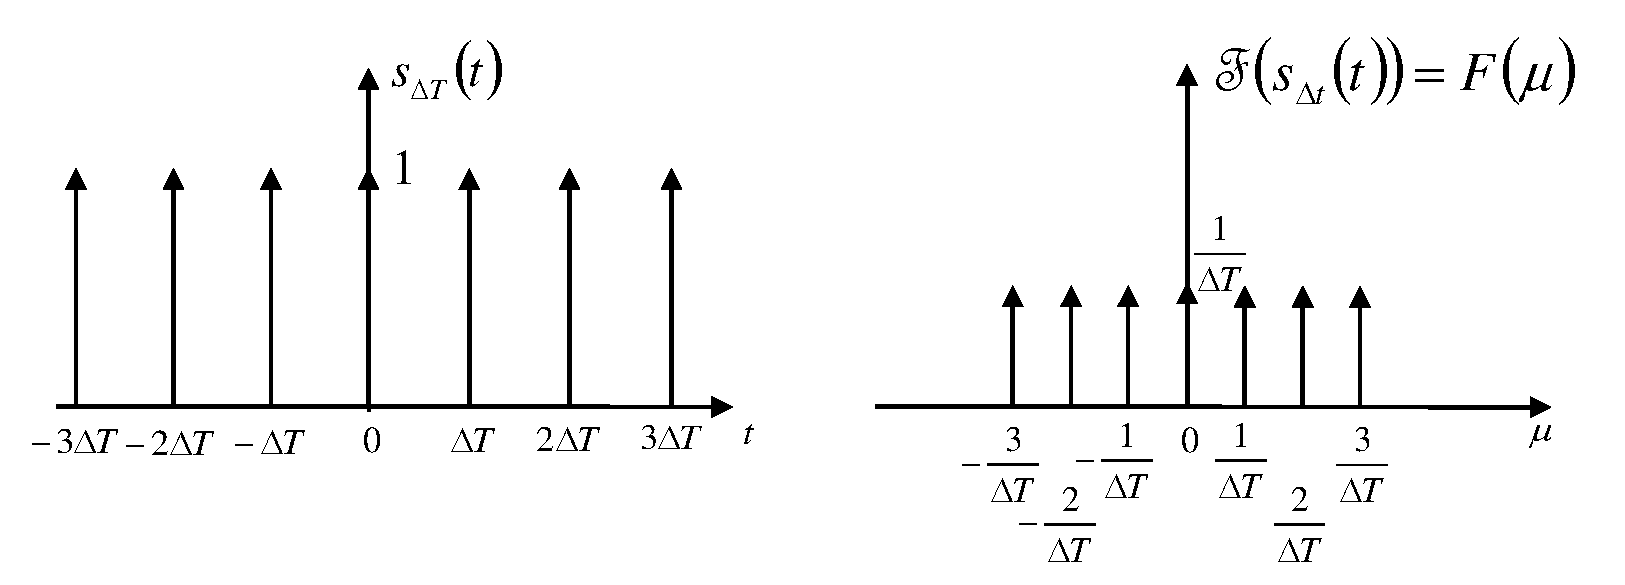
\includegraphics[scale=0.4]{5.pdf}
\end{center}

\paragraph*{Trasformata della convoluzione} La trasformata di Fourier della convoluzione è la seguente:
\begin{align*}
\mathfrak{F}[f * h](t) = H(\mu) \cdot F(\mu)
\end{align*}

\noindent Quindi:
\begin{itemize}
\item[-] La convoluzione di due segnali reali nel continuo diventa il prodotto delle loro trasformate;
\item[-] Il prodotto di due segnali reali nel continuo diventa la convoluzione delle loro trasformate.
\end{itemize}

\noindent Per questo motivo si tende ad eseguire il filtraggio sui segnali trasformati.
\end{document}